\documentclass[a4paper,12 pt]{article}
\usepackage[T1]{fontenc}
\usepackage{lmodern}
\usepackage[utf8]{inputenc}
\usepackage[italian]{babel}
\usepackage{booktabs}
\usepackage{color}
\usepackage{graphicx}
\usepackage{listings}
\usepackage{statrep}
\usepackage{emptypage}
\usepackage{newlfont}
\usepackage{enumerate}
\usepackage[hidelinks]{hyperref}
\usepackage[pass]{geometry}
\usepackage{titling}
\usepackage{hyperref}

\usepackage{listings}
\usepackage{color}

\setlength\parindent{0pt}
\definecolor{dkgreen}{rgb}{0,0.6,0}
\definecolor{gray}{rgb}{0.5,0.5,0.5}
\definecolor{mauve}{rgb}{0.58,0,0.82}
	
\lstset{
		language=Java,
		aboveskip=7mm,
		belowskip=7mm,
		showstringspaces=false,
		columns=flexible,
		basicstyle={\small\ttfamily},
		numbers=none,
		numberstyle=\tiny\color{gray},
		keywordstyle=\color{blue},
		commentstyle=\color{dkgreen},
		stringstyle=\color{mauve},
		breaklines=false,
		breakatwhitespace=true,
		tabsize=3
	}
\pagestyle{plain}

\title{Guida Java Console}
\author{Vittorio Valent \& Davide Ferretti}
\date{Giugno 2019}

\begin{document}
	\thispagestyle{empty}
	\begin{center}
		
\includegraphics[height=4cm]{Logo.png}
	\end{center}
	
	\maketitle
	\newpage
	\tableofcontents
	\newpage
	\section{Introduzione a Java}
	In questa breve guida esporremo le basi di Java e dei pattern utilizzati nel Training in Contrader. Questa guida non è una guida ufficiale ma solo un aiuto per coloro che si trovano in difficoltà all'inizio della loro esperienza da programmatori. Raccomandiamo di leggere attentamente il codice e i commenti (i quali rimandano proprio a questa guida). Per ogni domanda o suggerimento di ampliamento/modifica a questa guida potete mandare contattarci a\\
	
	\begin{itemize}
		\item  d.ferretti@contrader.it
		\item  v.valent@contrader.it
	\end{itemize}
	
	\noindent Java è un linguaggio di programmazione ad alto livello, orientato agli oggetti e a tipizzazione statica, che si appoggia sull'omonima piattaforma software, specificamente progettato per essere il più possibile indipendente dalla piattaforma hardware di esecuzione (tramite compilazione in bytecode prima e interpretazione poi da parte di una JavaVirtualMachine o JVM).\\
	
	\noindent Un programma minimale in Java deve obbligatoriamente contenere la definizione di classe tramite la parola chiave class seguita dal \textit{nomeclasse} e il metodo \textit{main} o metodo principale nonché entry point del programma in cui vengono definite variabili globali, oggetti e richiamati metodi statici su variabili e/o dinamici sugli oggetti.\\
	
	\begin{lstlisting}
		 class HelloWorld {
			public static void main(String[] args)
			{
				System.out.println("Hello World");
			}
		}
	\end{lstlisting}

	\noindent Nell'esempio soprastante il main contiene l'istruzione per la stampa a video della stringa Hello World; pur essendo perfettamente funzionante e semplice da comprendere, non viene sfruttata la filosofia ad oggetti che viene normalmente applicata ad ogni programma scritto in Java.\\
	Segue il codice sorgente di un programma che svolge lo stesso compito del precedente usando la programmazione orientata agli oggetti.
		\begin{lstlisting}
			public class Messaggio {
				private String toPrint;
			
				public Messaggio(String print) {
					this.toPrint = print;
				}
			
				public void print() {
					System.out.println(this.toPrint);
				}
			
				public static void main(String args[]) {
					Messaggio ciaoMondo = new Messaggio("Hello World!");
					ciaoMondo.print();
				}
			}
	\end{lstlisting}
	
	\noindent Il metodo main affida la stampa del messaggio a un oggetto creato apposta per questo compito, su cui è invocato il metodo dinamico \textit{print} definito prima del main assieme al costruttore della classe ovvero quel particolare metodo (con ugual nome della classe) che serve per inizializzare l'attributo della classe toPrint dell'oggetto creato/istanziato nel main.\\ I metodi definibili possono essere dichiarati \textit{privati} (contrassegnati dalla parola chiave private) se richiamabili solo all'interno della stessa classe oppure\textit{ pubblici} (contrassegnati dalla parola chiave \textit{public}) se richiamabili anche da altre classi, di tipo \textit{statico} (contrassegnati dalla parola chiave \textit{static}) se invocabili liberamente all'interno della classe (ad es. su variabili globali), dinamici se invocabili su oggetti.\\
	
	\noindent Scrivendo nuove classi che supportano l'operazione print, si può adattare il programma per mostrare messaggi di tipi radicalmente diversi, lasciando il main pressoché immutato, cambiando soltanto la metà riga che segue il new. Per esempio si può considerare un messaggio la scritta in una finestra che appare sullo schermo del computer in uso, oppure una stringa inviata su connessione di rete per apparire sulla finestra di un computer client. Oppure il programma può dialogare con l'utente sulla riga di comando (Java Console) o in una finestra (considerando il dialogo come un "messaggio interattivo").	
	
	\section{Classi e Oggetti}
	
	Java è un linguaggio\textit{ object-oriented}. L'idea che sta alla base della OOP è di rappresentare le entità reali o astratte che determinano le dinamiche del problema risolto dal software sotto forma di entità unitarie, dotate di specifiche d'uso e di funzionamento definite a priori. Queste entità sono chiamate \textit{oggetti}. Le specifiche che definiscono le caratteristiche di queste unità e in base a cui le stesse vengono create o, in gergo, \textit{istanziate}, sono chiamate classi.\\
	
	\noindent Java tuttavia non è un linguaggio ad oggetti puro, ma solamente object oriented (orientato agli oggetti): per esempio i valori dei tipi primitivi, come ad esempio \texttt{int}, \texttt{char} e \texttt{float},  non sono oggetti.
	
	\noindent Ogni classe di Java deve essere in un file separato che ha lo stesso nome della classe.È convenzione inoltre che i nomi delle classi comincino con la maiuscola, ed è bene rispettare questa prassi, per la leggibilità del codice, anche se non è obbligatoria. All'interno di una classe troveremo dei \textit{campi}, ovvero gli attributi della classe, uno o più costruttori per istanziare oggetti di questa classe ed eventualmente dei metodi (funzioni). \\
	
	\section{Metodi}
	
	Un metodo è un blocco di istruzioni che una classe o un oggetto rendono disponibili ad altre classi e/o oggetti, affinché possa essere eseguito su richiesta. \\
	In questo esempio, la JVM invoca il metodo main(), e questo metodo invoca il metodo scrivi(), il quale scrive una determinata stringa sulla console.
	
	\begin{lstlisting}
		public class Prova {
		
		public static void main(String[] args) {
		scrivi();
		}
		
		void scrivi() {
		System.out.println("prova");
		}
		
		}
	\end{lstlisting}
	\subsection{Composizione del metodo}
		L'intestazione di un metodo è definita da:
		\begin{itemize}
			\item eventuali modificatori
			\item tipo di ritorno
			\item nome del metodo
			\item lista di argomenti
		\end{itemize}
		I metodi sono utili perché permettono di definire dei "pacchetti" di istruzioni che vengono \textbf{eseguiti da un certo oggetto} su richiesta:
		
		\begin{lstlisting}
		public class Cane {
			
		public void abbaia() { System.out.println("Bau bau"); }
		public void dormi() { System.out.println("zzz"); }
			
		}
		
		public class Prova {
			public static void main(String[] args) {
			
			 	Cane c = new Cane();
			 	
				c.dormi();
				c.abbaia();
			}
		}
		\end{lstlisting}
	\subsection{Definire un metodo}
		La sintassi per l' implementazione (scrittura di codice) di un metodo è la seguente:
		\begin{lstlisting}
			modificatori tipo nomedelmetodo (parametri eventuali) {
			corpo del metodo;
		}
		\end{lstlisting}
		
		I parametri possono esserci oppure no.
		
		\noindent I metodi possono restituire un valore particolare al chiamante oppure no.\\ Quando si vuole restituire un valore il chiamante diverrà tale valore. La restituzione di un valore si ha con l'enunciato "return" ed il tipo del valore restituito indicato prima del nome del metodo. Se non si vuole restituire un valore o un dato particolare allora non occorre return e prima del nome del metodo c'è bisogno dell'enunciato "void". \\ Quindi, prima del nome del metodo, ci deve essere o il "void" o il tipo del valore (con all'interno del corpo la clausola "return").
		
	\section{Pattern MVC}
	
		Model-View-Controller (MVC), in informatica, è un pattern architetturale molto diffuso nello sviluppo di sistemi software, in particolare nell'ambito della programmazione orientata agli oggetti, in grado di separare la logica di presentazione dei dati dalla logica di business.
		
		\subsection{Componenti}
			Il componente centrale del MVC, il \textbf{Model}, cattura il comportamento dell'applicazione in termini di dominio del problema, indipendentemente dall'interfaccia utente. Il Model gestisce direttamente i dati (tramite il DAO) e le regole dell'applicazione con il Model (un'interessante metonimia che spesso genera confusione). \\
			
			\noindent Una \textbf{View} può essere una qualsiasi rappresentazione in output di informazioni, come ad esempio la stampa in Java Console. Sono possibili viste multiple delle stesse informazioni.\\
			
			\noindent La terza parte, il \textbf{Controller}, accetta l'input e lo converte in comandi per il Model e/o la Vista. Nel nostro caso è supportato da un Service che funge da collegamento con il Model.\\
		
		\subsection{Funzionamento}
			L'utente si interfaccia sempre con la View, che tramite un server web (nel nostro caso il famigerato \textit{MainDispatcher}, vedi il codice) che invia i dati e gli input al controller tramite \textit{Request} (pacchetti di informazioni a struttura chiave-valore, vedi codice).\\
			Il Controller usa i metodi del Service per ottenere ed elaborare i dati da rimandare alla View \textbf{sempre tramite Request}.\\
			
			\noindent Il Model infine definisce le entità dell'applicazione (nel Model, stessa confusione di prima) e interagisce con il \textit{Database}, recuperando e modificando i dati.\\
			
			\noindent Qui mostriamo in un diagramma le interazioni nel pattern MVC:\\
			
			
				\begin{center}
				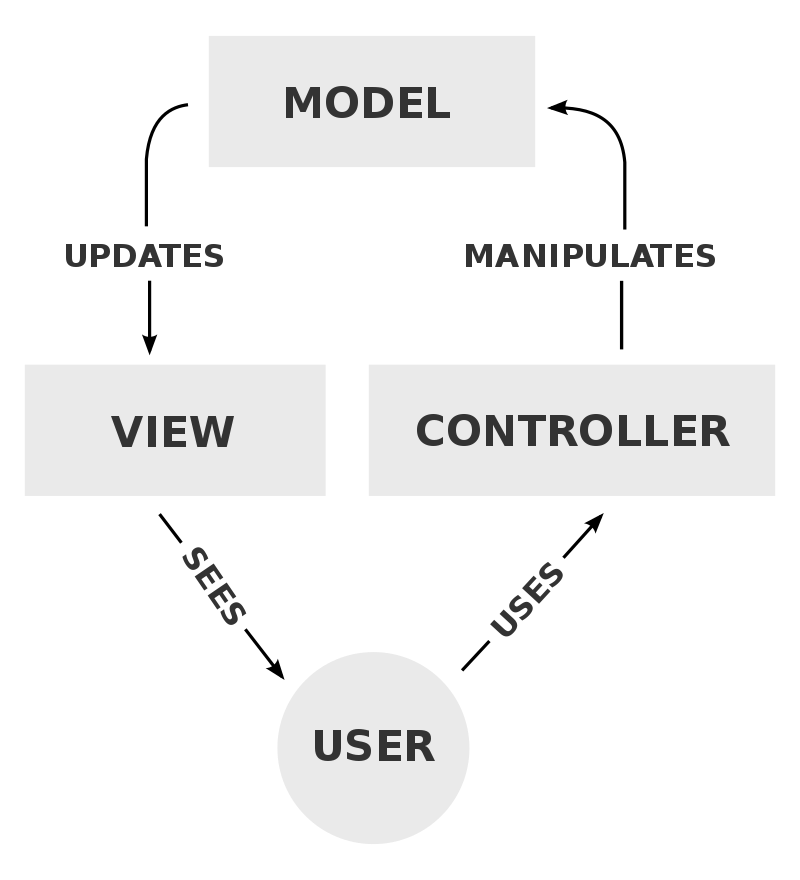
\includegraphics[height=8cm]{mvc.png}
			\end{center}
			
		
	\section{Model}
		Nel pacchetto model sono descritte tutte le entità dell'applicazione, ciascuna in una diversa classe. Ogni classe/entità possiede degli attributi, uno o più costruttori (in base al numero di argomenti), i metodi di accesso ai dati (Getter e Setter), un metodo per stampare l'oggetto in console (toString) e un metodo per il confronto degli oggetti (equals).\\
		In seguito analizziamo pezzo a pezzo le componenti della classe User del progetto SAPLEJava.
		\subsection{Attributi}
			I campi contrassegnati dal modificatore di accesso \texttt{private} sono i cosiddetti \textit{attributi} dell'entità. Avendo noi a che fare con un'entità di tipo User, avremo uno username, una password e un tipo di utente. Aggiungiamo inoltre un'id da usare come chiave privata sul database.\\
			
			\begin{lstlisting}	
				public class User {
				
					private int id;
					
					private String username;
					
					private String password;
					
					private String usertype;	
			\end{lstlisting}
			\subsection{Costruttore}
			Di seguito troviamo i due costruttori, uno per istanziare un oggetto senza attributi e uno che invece lo istanzia con tutti gli attributi (tranne l'id).
				\begin{lstlisting}
					public User() {
						// costruttore vuoto
					}
					
					public User (String username, String password, String usertype) {
						this.username = username;
						this.password = password;
						this.usertype = usertype;
					}	
				\end{lstlisting}
				
			\subsection{Getter e Setter}
			I metodi Getter e Setter servono alle altre classi ad accedere e modificare gli attributi di un oggetto. Infatti, a causa del modificatore di accesso \texttt{private}, le altre classi non potrebbero normalmente accedere a questi campi. Ci sono quindi due metodi per ogni attributo.\\
			 Il metodo get() non prende in pasto parametri e ritorna l'attributo.\\
			  Il metodo set(\textit{attributo}) non ha valore di ritorno e inserisce ( o sovrascrive) l'attributo all'interno dell'oggetto.
				\begin{lstlisting}
				public int getId() {
					return this.id;
				}
				public void setId(int id) {
					this.id = id;
				}
				
				public String getUsertype() {
					return this.usertype;
				}
				
				public void setUsertype(String usertype) {
					this.usertype = usertype;
				}
				
				public String getPassword() {
					return this.password;
				}
				
				public void setPassword(String password) {
					this.password = password;
				}
				
				public void setUsername(String username) {
					this.username = username;
				}
				
				public String getUsername() {
					return username;
				}
				\end{lstlisting}
				
				\subsection{ToString e Equals}
				
				Il metodo toString() restituisce l'oggetto trasformandolo in una stringa pronto alla stampa in Console. Il metodo equals controlla se due oggetti sono uguali (non essendo tipi primitivi non possono essere confrontati con un semplice '==').\\
				
				 Le annotazioni @Override segnala alla classe che i metodi devono sostituire i codici precedentemente presenti nei metodi (equals e toString sono presenti nella superclasse di User: Object).
				\begin{lstlisting}
				@Override
				public String toString() {
					return  id + "\t"  + username +"\t\t" +  
									 password + "\t\t" + usertype;
				}
				
				@Override
				public boolean equals(Object obj) {
					if (this == obj)
					return true;
					if (obj == null)
					return false;
					if (getClass() != obj.getClass())
					return false;
					User other = (User) obj;
					if (id != other.id)
					return false;
					if (password == null) {
						if (other.password != null)
						return false;
					} else if (!password.equals(other.password))
					return false;
					if (username == null) {
						if (other.username != null)
						return false;
					} else if (!username.equals(other.username))
					return false;
					if (usertype == null) {
						if (other.usertype != null)
						return false;
					} else if (!usertype.equals(other.usertype))
					return false;
					return true;
				}
			}
			\end{lstlisting}
	
	
	\section{DAO}
	Il livello del DAO (DAO è un pattern: Data Access Object) si occupa di recuperare le informazioni dal db. L'indirizzo del db è specificato nel file \texttt{config.properties}.
	Il DAO usa quindi una serie di query in linguaggio SQL che eseguirà sul database grazie ad una \textit{connessione} istanziata con il pattern \textit{Singleton}.\\
	
	In seguito analizziamo pezzo a pezzo il codice della classe "LoginDAO" del progetto SAMPLE.
	
	\subsection{Definizione della Query}
	I campi della classe DAO sono delle stringhe che rappresentano le query da inoltrare al database. Dato che queste non devono essere modificabili in runtime le dotiamo di modificatore \texttt{final}. In questo caso eseguiamo una query che risultato restituirà uno user i cui attributi corrispondono a quelli da noi forniti (che verranno inseriti dal programma al posto del punto interrogativo).
	\begin{lstlisting}
	public class LoginDAO {
		
		private final String QUERY_LOGIN = "SELECT * FROM user 
										WHERE username = ? AND password = ?";
	\end{lstlisting}
	
	\subsection{Connessione al DB}
	La query viene eseguita all'interno di un metodo (nel nostro caso il metodo \texttt{login()}) attraverso una \textit{connessione} al database.\\
	La connessione a database viene istanziata seguendo il pattern Singleton (metodo \texttt{getIstance()} ). Successivamente, tramite il metodo \texttt{prepareStatement} di Connection impostiamo la query che vogliamo eseguire e gli eventuali parametri (in questo caso username e password). L'oggetto ResultSet verrà riempito dai dati ottenuti dalla query in seguito. Il costrutto \texttt{ try - catch} è obbligatorio e serve a evitare che il programma fallisca nel caso in cui la query non andasse a buon fine.
	
	\begin{lstlisting}
		public String login (String username, String password) {
		
		Connection connection = ConnectionSingleton.getInstance();
			
			try {
				PreparedStatement statement = connection
								.prepareStatement(QUERY_LOGIN);
			
					statement.setString(1, username);
					statement.setString(2, password);
	
					ResultSet resultSet;
	\end{lstlisting}
	
	\subsection{Esecuzione della Query}
	Se l'esecuzione della Query è andata a buon fine resultSet diventa il risultato della query (in questo caso avremo uno user scomposto come "username", "password", "usertype" e "id")
	Da questo estraiamo il valore sotto la chiave "usertype" e lo incapsuliamo nella variabile usertype che poi ritorniamo. In caso di errore nella query entreremo nel \texttt{catch} e avremo un valore di ritorno nullo.
	\begin{lstlisting}
				if(statement.executeQuery().next()) {
				
					String usertype = null;
					
					resultSet = statement.executeQuery();
					resultSet.next();
					usertype = resultSet.getString("usertype");
				}
		
					return usertype;
			}
		
			catch (SQLException e) {
				return null;
			}
		}
	}
	\end{lstlisting}
\clearpage

	\section{Service}
	I Service svolgono la funzione da tramite tra i Controller (che li invocano) e i DAO (invocati dal Service). Nella versione SAMPLEJavaPRO i Service chiamano i Converter che trasformano i dati del Model in DTO (vedi Guida Java Console Pro).\\
	
	Per invocare i metodi del DAO istanzia un oggetto di tipo LoginDAO nel costruttore della classe:
	\begin{lstlisting}
	public class LoginService {
	
		private LoginDAO loginDAO;

		public LoginService() {
			this.loginDAO = new LoginDAO();
		}
	\end{lstlisting}
	
	Successivamente usa questo oggetto nel metodo login per invocare il metodo login (di loginDAO) passando come parametri lo username e la pasword.
	\begin{lstlisting}
		public String login (String username, String password) {
			return this.loginDAO.login(username, password);
		}
	}	
	\end{lstlisting}
	
	\section{Controller}
	I Controller rappresentano il collegamento tra l'applicazione e la View: essi infatti invocano i Service per ottenere e/o manipolare dati e li inviano alla View tramite Request\footnote{ATTENZIONE: Le View non possono invocare i metodi del controller ma possono solo ricevere oggetti di tipo request tramite il MainDispatcher!}.\\
	
	Vediamo ora nel dettaglio come funziona il LoginController del progetto SAMPLE.
	\subsection{Interfaccia Controller}
	Innanzitutto osserviamo che ogni Controller implementa l'interfaccia Controller: ciò significa che ogni classe Controller è \textit{obbligata} ad implementare il metodo \texttt{doControl()}. Questo controller necessita inoltre di costruire un oggetto di tipo LoginService per utilizzare i metodi del LoginService.

	\begin{lstlisting}
		public class HomeController implements Controller {
		
			private LoginService loginService;
	
			public HomeController() {
			loginService = new LoginService();
			}
	\end{lstlisting}
	
	\subsection{Metodo doControl}
	Il metodo \texttt{doControl()} è il metodo principale del Controller. Esso ha come unico parametro una Request, ovvero un pacchetto di informazioni ad accesso ("chiave", valore). Il metodo generalmente controlla che la richiesta non sia nulla, quindi la \textit{spacchetta} estraendo con request.get("chiave") i valori al suo interno (di tipo Object). Il \texttt{toString()} serve solo a trasformare questi Object in stringhe. Ottenuti questi dati (che arrivano dalla LoginView) invoca il metodo del Service che restituisce la stringa \texttt{usertype}.
	\begin{lstlisting}
			public void doControl(Request request) {
				if (request != null) {
			
				String username = request.get("username").toString();
				String password = request.get("password").toString();
	
				String usertype= loginService.login(username, password);
		\end{lstlisting}
	\subsection{Reindirizzare ad una View}
	Il metodo ora esegue uno switch case in base allo usertype ottenuto. Se lo usertype è "ADMIN" il controller reindirizza, tramite il MainDispatcher e il metodo \texttt{callView("NomeView), request)}, alla Home dell'admin; se è
	"USER" il controller manda alla Home dello user. Se lo usertype non è uno di questi o se la request è nulla si ritorna alla pagina di Login.
		\begin{lstlisting}	
					switch(usertype) {
				
					case "ADMIN":
						MainDispatcher.getInstance().callView("HomeAdmin", request);
						break;
				
					case "USER": 
						MainDispatcher.getInstance().callView("HomeUser", request);
						break;
				
					default:
						MainDispatcher.getInstance().callView("Login", null);
						break;
					}
				}
				else MainDispatcher.getInstance().callView("Login", null);
			}
		}
	\end{lstlisting}
	\section{View}
	Le View si occupano di stampare in console dati, messaggi e opzioni. Ovviamente la grafica di un'applicazione JavaConsole non sarà particolarmente sofisticata per evitare di complicare inutilmente le classi. Osserviamo che questa classe estende AbstractView (dove è implementato il metodo \texttt{getInput()}) che a sua volta implementa l'interfaccia View. Quest'ultima firma tre metodi: 
	\begin{itemize}
		\item \texttt{showResult()};
		\item \texttt{showOption()};
		\item \texttt{submit()}
	\end{itemize}
	Vedremo più avanti cosa fanno esattamente questi metodi nella loro implementazione.
	\begin{lstlisting}
	public class LoginView extends AbstractView {
	
		private String username;
		
		private String password;
	\end{lstlisting}
	
	\subsection{Metodo showResults}
	Il metodo \texttt{showResults()} mostra i dati che arrivano dal controller nella request (ad esempio una lista di DTO). In questo caso, non essendoci nulla da mostrare, 
	il corpo è vuoto. Se si vuole skippare questo metodo arrivando dal controller basta mettere all'interno del metodo un \texttt{if} che controlla se la request con i dati da mostrare ) e nulla o meno\footnote{Vedi UserReadView}.
	\begin{lstlisting}	
		public void showResults(Request request) {
		
		}
	\end{lstlisting}
	
	\subsection{Metodo showOptiosn}
	Il metodo \texttt{showOptions()} svolge il ruolo di "menù" della View, proponendo una o più scelte da inserire da tastiera. Il metodo che si occupa di prendere in
	input un dato è \texttt{getInput()}.
	\begin{lstlisting}	
		public void showOptions() {
		
			System.out.println("----- .:LOGIN:. ----");
			
			System.out.println(" Nome utente:");
			this.username = getInput();
			
			System.out.println(" Password:");
			this.password = getInput();
		}
	\end{lstlisting}
		
		\subsection{Metodo submit}
		La funzione del metodo \texttt{submit()}, come suggerisce il nome, è quello di prendere i dati inseriti dall'utente, impacchettarli in una \textbf{nuova} Request e inviarli al controller
		tramite il MainDIspatcher.
		\begin{lstlisting}
		public void submit() {
			
			Request request = new Request();
			
			request.put("username", username);
			request.put("password", password);
			
			MainDispatcher.getInstance().callAction("Home", "doControl", request);
		}
	
	
	}
	\end{lstlisting}
	
	\section{Pattern Singleton}
	Il singleton è un design pattern creazionale che ha lo scopo di garantire che di una determinata classe venga creata una e una sola istanza, e di fornire un punto di accesso globale a tale istanza.\\
	
	L'implementazione più semplice di questo pattern prevede che la classe singleton abbia un unico costruttore privato, in modo da impedire l'istanziazione diretta della classe. La classe fornisce inoltre un metodo "getter" statico che restituisce l'istanza della classe (sempre la stessa), creandola preventivamente o alla prima chiamata del metodo, e memorizzandone il riferimento in un attributo privato anch'esso statico \\
	
	Di seguito troviamo una semplice implementazione:
	\begin{lstlisting}
	public class Singleton {
		
		private static Singleton istance = null;
			
		//Il costruttore private impedisce
		// l'istanza di oggetti da parte di classi esterne
		private Singleton() {
		}
		
		// Metodo della classe impiegato
		// per accedere al singleton
		public static Singleton getIstance() {
			if (istance == null) {
				istance = new Singleton();
			}
			return istance;
		}
	}
	\end{lstlisting}
	
\end{document}